\documentclass[11pt]{article}

\usepackage{multirow}
\usepackage[margin=3cm]{geometry}
\usepackage{hyperref}
\usepackage{amsmath}

\title{Relatório Trabalho Técnologias Web}
\author{Luís Maurício - 37722\\Fábio Macarrão - 37814\\}
\date{2020/2021}

\usepackage{graphicx}
\begin{document}
	\pagenumbering{gobble}
	\maketitle

	\newpage
	\pagenumbering{arabic}
	\section{Geral}
	\subsection{HTML}
	\paragraph{}
	Código adicionado a todos os ficheiros html acessiveis. 
	
	\begin{figure}[htp]
\centering
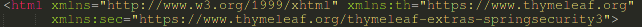
\includegraphics[scale=0.75]{html.png}
\caption{Import da segurança}
\label{}
\end{figure}
	
\begin{figure}[htp]
\centering
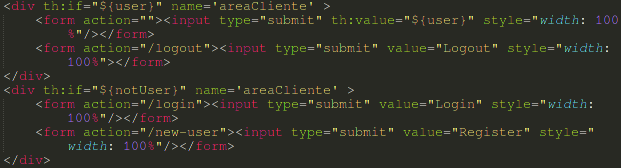
\includegraphics[scale=0.75]{botoes.png}
\caption{Botões para login/logout}
\label{}
\end{figure}

\begin{figure}[htp]
\centering
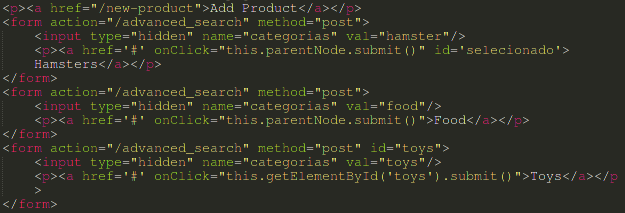
\includegraphics[scale=0.75]{filtro.png}
\caption{Filtro por categoria do produto}
\label{}
\end{figure}
	
\newpage
	
\section{Criar Utilizador}
	\subsection{Utilizador.java}
	\paragraph{}
	Modelo que contém o objecto Utilizador com os atributos u\_id (atribuido automaticamente), username, password, email, uma lista de Encomenda e um role. Os dados para o registo de novo utilizador são preenchidos na página new-user.html, após a página ser mapeada em NovoUtilizadorController.java.  

	\subsection{NovoUtilizadorController.java}
	\paragraph{}
	Faz o GetMapping para carregar a página new-user.html e o PostMappping para registar os utilizadores na base de dados utilizando o UtilizadorRepo.java.

	\subsection{UtilizadorRepo.java}
	\paragraph{}
	Repositório responsável pela gestão de utilizadores, realizando as operações CRUD sobre a base de dados.
	
\section{Criar Produto}	
	\subsection{Produto.java}
	\paragraph{}
	Contém o objecto Produto com os atributos p\_id (atribuido automaticamente), nome, imag, descr, categoria e preco. Os dados para o registo de novo produto são preenchidos na página new-product.html, após a página ser mapeada em NovoProdutoController.java. 
	
	\subsection{NovoProdutoController.java}
	\paragraph{}
	Faz o GetMapping da  para carregar a página new-product.html e o PostMappping para registar os produtos na base de dados utilizando o ProdutoRepo.java.
	
	\subsection{ProdutoController.java}
	\paragraph{}
	Faz o GetMapping para carregar a página product.html e o PostMappping para aceder aos produtos na base de dados utilizando o ProdutoRepo.java.
	
	\subsection{AdvancedSearchController.java}
	\paragraph{}
	Faz o GetMapping para carregar a página advanced_search.html e o PostMapssing para aceder aos produtos na base de dados utilizando o ProdutoRepo.java.

	\subsection{SearchController.java}
	\paragraph{}
	Faz o GetMapping para carregar a página search.html e o PostMappping para aceder aos produtos na base de dados utilizando o ProdutoRepo.java.

	\subsection{ProdutoRepo.java}
	\paragraph{}
	Repositório responsável pela gestão dos produtos, realizando as operações CRUD sobre a base de dados.
	
\section{Criar Encomenda}
	\subsection{Encomenda.java}
	\paragraph{}
	Contém o objecto Encomenda com os atributos e\_id (atribuido automaticamente), Utilizador e DetalhesEncomenda. Os dados para o registo de uma encomenda são preenchidos no index.html, através de um botão adicionar para acrescentar o produto ao carrinho, após a página ser mapeada em EncomendaController.java.
	
	\subsection{EncomendaController.java}
	\paragraph{}
	Faz o GetMapping para carregar a página list-order.html e o PostMappping para aceder aos produtos na base de dados utilizando o DetalhesEncomendaRepo.java.
	
	\subsection{DetalhesEncomenda.java}
	\paragraph{}
	Contém o objecto DetalhesEncomenda com os atributos d\_id (atribuido automaticamente), Encomenda, produto\_id e quantidade. Os dados da encomenda podem ser visualizados em list-order.html, após a página ser mapeada em ListEncomendaController.java.

	\subsection{ApagaProdutoController.java}
	\paragraph{}
	Faz o GetMapping para carregar a página del-product.html e o PostMappping para apagar produtos da base de dados ou da lista de compras, utilizando UtilizadorRepo.java ou ProdutoRepo.

	\subsection{EncomendaRepo.java}
	\paragraph{}
	Repositório responsável pela gestão das encomendas, realizando as operaçoes CRUD sobre a base de dados.

	\subsection{DetalhesEncomendaRepo.java}
	\paragraph{}
	Repositório responsável pela gestão dos detalhes das encomendas, realizando as operaçoes CRUD sobre a base de dados.
	
\section{Controlo}
	\subsection{MainController.java}
	\paragraph{}
	Responsável por controlar a açao de logout e ainda servir a view de login e index.

	
\section{Configurações}
	\subsection{WebSecurityConfig.java}
	\paragraph{}
	Configurações de autenticaçao e de autorizaçao dos utilizadores.

\section{Excepções}
	\subsection{StorageException.java}
	\paragraph{}
	Mostra uma mensagem sempre quando o upload falha.

\section{Serviços}
	\subsection{StorageService.java}
	\paragraph{}
	Permite fazer o upload de ficheiros externos à WebApp (neste caso imagens).

 	\subsection{UserDetalhesServiceImpl.java}
	\paragraph{}
	Serviço que le um utilizador da base de dados e cria um objecto MyUserDetails para associar uma GrantedAuthority a cada utilizador.

\section{Outros}
	\subsection{MyUserDetails.java}
	\paragraph{}
	Associa uma Collection<rantedAuthority> ao utilizador a partir do campo role. GrantedAuthority é utilizada para implementaçao de autorizaçao.

	\subsection{XhamsterApplication.java}
	\paragraph{}
	Corre a WebApp.


	
\end{document}